\documentclass[a4paper, oneside]{book}
\usepackage[italian]{babel}
\usepackage[utf8]{inputenc}
\usepackage[a4paper,top=2.5cm,bottom=2.5cm,left=2cm,right=2cm]{geometry}
\usepackage{amssymb}
\usepackage{amsthm}
\usepackage{graphics}
\usepackage{amsfonts}
\usepackage{amsmath}
\usepackage{amstext}
\usepackage{engrec}
\usepackage{rotating}
\usepackage[safe,extra]{tipa}
\usepackage{multirow}
\usepackage{hyperref}
\usepackage{enumerate}
\usepackage{braket}
\usepackage{marginnote}
\usepackage{pgfplots}
\usepackage{cancel}
\usepackage{polynom}
\usepackage{booktabs}
\usepackage{enumitem}
\usepackage{algorithm}
\usepackage{algpseudocode}
\usepackage{framed}
\usepackage{pdfpages}
\usepackage{pgfplots}
\usepackage{fancyhdr}
\usepackage{caption}
\usepackage{subcaption}
\usepackage{setspace}
\usepackage{hyperref}
\pagestyle{fancy}
\fancyhead[L,RO]{\slshape \rightmark}
\fancyfoot[C]{\thepage}

\title{Causal Networks}
\author{Tommaso Ferrario (\href{https://github.com/TommasoFerrario18}{@TommasoFerrario18})}
\date{Ottobre 2024}

\pgfplotsset{compat=1.13}

\begin{document}

\maketitle
\newtheorem{teorema}{Teorema}
\newtheorem{dimostrazione}{Dimostrazione}
\newtheorem{definition}{Definition}
\newtheorem{esempio}{Esempio}
\newtheorem{osservazione}{Osservazione}
\newtheorem{note}{Note}
\newtheorem{corollario}{Corollario}
\tableofcontents
\renewcommand{\chaptermark}[1]{
    \markboth{\chaptername
        \ \thechapter.\ #1}{}}
\renewcommand{\sectionmark}[1]{\markright{\thesection.\ #1}}

\chapter{Potential outcomes}
In the following course we will use the following notation:
\begin{itemize}
    \item $X$ to denote the random variable representing the \textbf{treatment}
          assignment.
    \item $Y$ to denote the random variable representing the \textbf{outcome} of
          interest.
    \item $Z$ to denote a set of random variables representing \textbf{covariates}.
\end{itemize}

Also, we will use uppercase letters to denote random variables and lowercase
letters to denote their realizations.

\begin{definition}[Potential outcomes]
    $Y(x)$ denotes what your outcome would be, if you were to take treatment $X = x$.
\end{definition}
A \textbf{potential outcome} $Y(x)$ is distinct from the \textbf{observed outcome} $Y$ in that not
all potential outcomes are observed. But, all potential outcomes can potentially
be observed but we can't observe potential outcome of a decision that isn't made.

The actually observed outcome depends on the given value $x$ of treatment $X$.
The potential outcome is the value of $Y$ before making the decision of the
treatment $X=x$.

Up until now, we have been considering an individual. However, the population
consists of many individuals. Each individual is tipically associated with one or
more variables, referred to as covariates $Z$. We denote each individual using $i$
as as subscript.

\begin{definition}[Individual treatment effect]
    The individual treatment effect (ITE) for the $i^{th}$ individual
    is defined as the difference between the potential outcomes:
    \begin{equation}
        \tau_i \triangleq Y_i(1) - Y_i(0)
    \end{equation}

    The main different is that $Y(x)$ is a random variable because different individuals
    have different potential outcomes. Meanwhile, $Y_i(x)$ is a treated as a
    non-random variable because it is the potential outcome is deterministic, because
    it is conditioned by $i$-individual.
\end{definition}

\begin{note}
    If the individual treatment effect is different from zero, we can call it
    the \textbf{causal effect} of the treatment. Otherwise, we can call it the
    \textbf{no causal effect}.
\end{note}

\section{Fundamental problem of causal inference}
As we said before, it's impossible to observe all potential outcomes for a given
individual. Therefore, we can't observe the causal effect:
\begin{equation*}
    \tau_i \triangleq Y_i(1) - Y_i(0)
\end{equation*}

The potential outcome that you don't observe are known as \textbf{counterfactuals}.
So, a potential outcome $Y(x)$ doesn't become counterfactual until another
potential outcome $Y(x')$ is observed.

\begin{note}
    There are no counterfactuals or factuals until the outcome is observed.
\end{note}
\begin{definition}
    The \textbf{average treatment effect} (ATE) is obtained by taking an average
    over the individual treatment effects:
    \begin{equation}
        \tau \triangleq \mathbb{E}[\tau_i] = \mathbb{E}[Y_i(1) - Y_i(0)] = \mathbb{E}[Y(1) - Y(0)]
    \end{equation}
    where we recall that the average is over the individuals $i$ if $Y_i(x)$ is
    deterministic.
\end{definition}

The fundamental problem can be see as a missing data problem. Therefore, we cannot
compute directly the average treatment effect. We could be tempted to use the
associational difference:
\begin{equation}
    \mathbb{E}[Y|X = 1] - \mathbb{E}[Y|X = 0]
\end{equation}

Unfortunately, this is not true in general to compute the average treatment effect.
Because $\mathbb{E}[Y|X = 1] - \mathbb{E}[Y|X = 0]$ is an associational quantity,
while $\mathbb{E}[Y(1)] - \mathbb{E}[Y(0)]$ is a causal quantity.

In general, they are not equal due to the \textbf{confounding} effect of the covariates
$Z$. For example, using the representation in figure \ref{fig:confounding} we can
say that the covariate $Z$ confounds the effect of $X$ on $Y$, because of the
following path:
\begin{equation*}
    X \rightarrow Y \leftarrow Z
\end{equation*}

\begin{figure}[!ht]
    \centering
    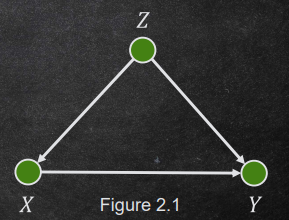
\includegraphics[width=0.35\textwidth]{img/confounding.png}
    \caption{Confounding effect of the covariate $Z$}
    \label{fig:confounding}
\end{figure}

We can consider average treatment effect equal to the associational difference
assuming the \textbf{ignorability} assumption.
\begin{definition}[Ignorability]
    The \textbf{ignorability} assumption states that the treatment assignment
    is random and independent of the potential outcomes:
    \begin{equation}
        Y(0), Y(1) \perp X
    \end{equation}
\end{definition}

Another name for this property is \textbf{exchangeability} because it can be
interpreted as we can exchange \textbf{treatment} and \textbf{control} groups without changing the
distribution of the potential outcomes.

In graphical sense, we can see the same structure of figure \ref{fig:confounding}
but without $Z \to X$ path.

We can distinguish between two types of ignorability:
\begin{itemize}
    \item \textbf{Mean ignorability}:
          \begin{equation*}
              \mathbb{E}[Y(1)|X = x]  =  \mathbb{E}[Y(1)]\ \ \ \
              \mathbb{E}[Y(0)|X = x]  =  \mathbb{E}[Y(0)] \ \forall x \in X
          \end{equation*}
    \item \textbf{Full ignorability}:
          \begin{equation*}
              (Y(1), Y(0))\perp X
          \end{equation*}
\end{itemize}
In general, mean ignorability is enough to compute the average
treatment effect.

This property is fundamental because it allows us to compute the average treatment
effect as the associational difference:
\begin{equation*}
    \tau \triangleq \mathbb{E}[Y(1) - Y(0)] = \mathbb{E}[Y|X = 1] - \mathbb{E}[Y|X = 0]
\end{equation*}

The assumption of ignorability allow us to identify causal effects. This can be
done reducing a causal expression to a purely statistical expression. We can
calculate the causal effect from just the observational distribution $P(X, Y, Z)$.

\begin{definition}[Identifiability]
    A causal quantity is identifiable if we can compute it from a purely statistical
    quantity.
\end{definition}

Unfortunately, the assumption of ignorability is completely unrealistic, confounding
is likely to happen in most data we observe. We can make the assumption of ignorability
more realistic by performing a \textbf{randomized experiment}, which force the treatment
$X$ to be cause randomly solving the problem of the confounding effect.

In observational data, it's unrealistic to assume that the groups are exchangeable.
However, if we control for relevant variables by conditioning, then maybe the groups
will be exchangeable.

\begin{definition}[Conditional exchangeability]
    The \textbf{conditional exchangeability} or \textbf{unconfoundeness} assumption
    states that the treatment assignment is the potential outcomes conditional
    on the covariates:
    \begin{equation}
        Y(0), Y(1) \perp X | Z
    \end{equation}
\end{definition}

Indeed, when conditioning on $Z$, non-causal associations between $X$ and $Y$ no
longer exists. Non-causal association is blocked by conditioning on $Z$.

This is the main assumption necessary for use the causal inference. We can now identify
the causal effect within levels of $Z$, just like we did with ignorability:
\begin{equation}
    \mathbb{E}[Y(1) - Y(0) | Z] = \mathbb{E}[Y(1)| Z] - \mathbb{E}[Y(0)| Z] =
    \mathbb{E}[Y|X = 1, Z] - \mathbb{E}[Y|X = 0, Z]
\end{equation}

If we want the marginal effect that we had before when assuming ignorability, we
can get that by simply marginalizing over $Z$ as follows:
\begin{equation}
    \mathbb{E}[Y(1) - Y(0)] = \mathbb{E}_Z[\mathbb{E}[Y(1) - Y(0) | Z]]
\end{equation}

\begin{definition}[Adjustment formula]
    Given the assumption of \textbf{unconfoundeness}, \textbf{positivity}, \textbf{consistency}, and \textbf{no interference},
    we can identify the average treatment effect as:
    \begin{equation}
        \tau = \mathbb{E}[Y(1) - Y(0)] = \mathbb{E}_Z[\mathbb{E}[Y(1) - Y(0) | Z]]
        = \mathbb{E}_Z[\mathbb{E}[Y|X = 1, Z] - \mathbb{E}[Y|X = 0, Z]]
    \end{equation}
\end{definition}

In the adjusted formula we moved from the assumption of ignorability to that
of unconfoundedness because it seems more realistic. However, we often cannot know for certain if unconfoundedness holds.

There may be some \textbf{unobserved confounders} that we can't control, this mean that
the assumption of unconfoundeness is violated. The best we can do is to observe
and fit as many covariates as possible to try to ensure unconfoundeness.

\begin{note}
    that is not the case for randomized experiment.
\end{note}

Indeed, it can be the case we obtain more biased estimates by including when
adjusting for the "wrong" covariates.

\begin{definition}[Positivity]
    Positivity is the condition that all the subgroups af the data with different
    value $z$ for covariates $Z$ have some probability of receiving treatment $X$.

    For all values $z$ of covariates $Z$ present in the population of interest,
    we have:
    \begin{equation}
        0 < P(X = 1 | Z = z) < 1, \forall z
    \end{equation}
\end{definition}

If we have positivity violation, then we will be conditioning on a \textbf{zero probability}
event. This will lead to biased estimates. Infact, we will have a division by $0$.

Positivity is also referred to as the \textbf{overlap} assumption. This is because
we want the covariates distribution of the group to overlap.

\begin{figure}[!ht]
    \centering
    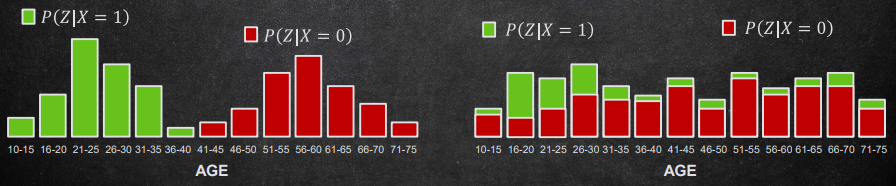
\includegraphics[width=\textwidth]{img/overlap.png}
    \caption{Example of overlap}
    \label{fig:positivity}
\end{figure}

Adjusting on a lot of covariets can lead to \textbf{curse of dimensionality}, because
all the subgrup can be contained in the control group or in the treatment group.

Another important assumption is the \textbf{no interference} assumption.
\begin{definition}[No interference]
    The outcome $Y_i$ of the $i^{th}$ individual is not affected by anyone else's
    treatment $X_j$ for $j \neq i$.
    \begin{equation}
        Y_i(x_1, x_2, \ldots, x_i, \ldots, x_n) = Y_i(x_i)
    \end{equation}
\end{definition}

The last assumption is the \textbf{consistency} assumption.
\begin{definition}[Consistency]
    If the treatment is $X$, then the observed outcome $Y$ is the potential outcome
    under treatment $X$. Formally:
    \begin{equation}
        X = x \rightarrow Y = Y(X)
    \end{equation}
\end{definition}

We need the treatment to be well defined, if consistency is not respected $Y(1)$
is not well defined since it will be $1$ or $0$ and it depends on something that
is not captured  by the treatment $X$.

\begin{definition}[Stable Unit Treatment Value Assumption]
    The \textbf{Stable Unit Treatment Value Assumption} (SUTVA) is satisfied if
    individual $i$'s outcome $Y_i$ is simply a function of the treatment $X_i$.
\end{definition}

SUTVA is a combination of consistency, no interference and deterministic potential
outcome.

Now, we need to introduce some terminology that will be useful in the following
chapters.
\begin{itemize}
    \item \textbf{Estimand}: The quantity that we want to estimate.
    \item \textbf{Estimate}: an approximation of the estimand, which we get
          using data.
    \item \textbf{Estimator}: a function that maps the data to an estimate of the
          estimand.
    \item \textbf{Estimation}: the process that we use to go from data plus the
          estimand to a concrete number is known as estimation.
    \item \textbf{Causal estimand}: refers to any estimand that contains a potential
          outcome in it.
    \item \textbf{Statistical estimand}: refers to any estimand that does not contain
          a potential outcome in it.
\end{itemize}

The process of estimation is shown in figure \ref{fig:pipeline}. We need to
introduce also the concept of \textbf{identification}, which is the process of
moving a causal estimand to an equivalent statistical estimand. And the concept
of \textbf{Estimation}, which is the process of moving from a statistical estimand
to an estimate.
\begin{figure}[!ht]
    \centering
    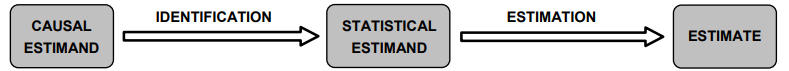
\includegraphics[width=\textwidth]{img/process.png}
    \caption{Process of estimation}
    \label{fig:pipeline}
\end{figure}

When we want to answer to causal estimand, so a question thet we want to answer when
we do something so we interactive, we want to pass to a statistical estimand
to prove our answer using observation datas and this process of passing from causal
estimand to statistical estimand is called identification. Not always is possible
to do identification. When exist identification, we can answer an intervational query
without intervening on the experiment.

To do identification we need a causal model, so we define some assumption on causal
relationship between variables and this define if a causal estimand could be translate
in a statistical estimand.

Generaly in AI everyone wants to take decision using observation estimand computed
on data, but these are all subjected to bias.
\chapter{Flow of Association}
Assume we only care about modeling association, without any causal modeling. If
we want to model the data distribution $P(X_1, X_2, \ldots, X_n)$, we can use
the chain rule of probability to decompose it into a product of conditional
distributions:
\begin{equation}
    P(X_1, X_2, \ldots, X_n) = P(X_1)P(X_2|X_1)P(X_3|X_1, X_2)\ldots P(X_n|X_1, X_2, \ldots, X_{n-1})
\end{equation}
However, if we were to model discrete random variables by using probability
tables, it would take an exponential number of parameters. To solve this we
can model local dependencies between variables to reduce the number of
parameters.

\begin{definition}[\textbf{Local Markov Assumption}]
    Given all the parents $pa(x)$ of a node $x$ in a DAG, the local Markov
    assumption states that $x$ is independent of all its non-descendants.
\end{definition}
Talking about Bayesian networks, the local Markov assumption is equivalent to
the \textbf{bayesian network factorization}:
\begin{equation}
    P(X_1, X_2, \ldots, X_n) = \prod_{i=1}^n P(X_i|pa(X_i))
\end{equation}

At this point we can define a \textbf{markov probability distribution} as a
probability distribution $P$ that satisfies the local Markov assumption with
respect to a DAG $G$.

As important as the local Markov assumption is, it only gives us information
about the independencies in $P$ that a DAG $G$ implies.

To get this guaranteed dependence between adjacent nodes, we will generally
assume a slightly stronger assumption than the local Markov assumption, called
the \textbf{minimality assumption}.
\begin{definition}[\textbf{Minimality Assumption}]
    The minimality assumption means:
    \begin{enumerate}
        \item \textbf{local markov assumption}: Given all the parents $pa(x)$ of
              a node $x$ in a DAG, the local Markov assumption states that $x$
              is independent of all its non-descendants.
        \item Adjacent nodes in the DAG $G$ are dependent.
    \end{enumerate}
\end{definition}

Because removing edges in a Bayesian network is equivalent to adding
independencies, the minimality assumption is equivalent to saying that we can't
remove any more edges from the graph $G$.

\begin{definition}
    $P$ and $G$ are Markov Compatible if $P$ factorize according to $G$. 
\end{definition}

Up to now all we presented was about statistical models and modeling association.
We now need to introduce some causal assumptions, turn them into causal models
for allowing the study of causation. In order to introduce causal assumptions,
we must first understand what it means for $X$ to be a cause of $Y$. We can simply
define \textbf{cause} as follows:
\begin{definition}[\textbf{Cause}]
    $X$ is a cause of $Y$ if changing $X$ changes $Y$.
\end{definition}

Also, we can define \textbf{(strict) causal edges assumption} in a DAG $G$ as every parent
is a direct cause of all its children. Given this assumption, we can define a
\textbf{Causal graph} as a DAG $G$ that satisfies the causal edges assumption.

Adding the causal edges assumption, implies that directed paths in the DAG take
on a very special meaning; they correspond to \textbf{causation}. This is in
contrast to other paths in the graph, which association may flow along, but
causation certainly may not.
\section{Basic Structure}
To understand the difference between association flow and causal flow in DAGs,
we need the following minimal building blocks
\begin{itemize}
    \item chain
    \item fork
    \item collider
    \item two un-connected nodes
    \item two connected nodes
\end{itemize}
\begin{figure}[!ht]
    \centering
    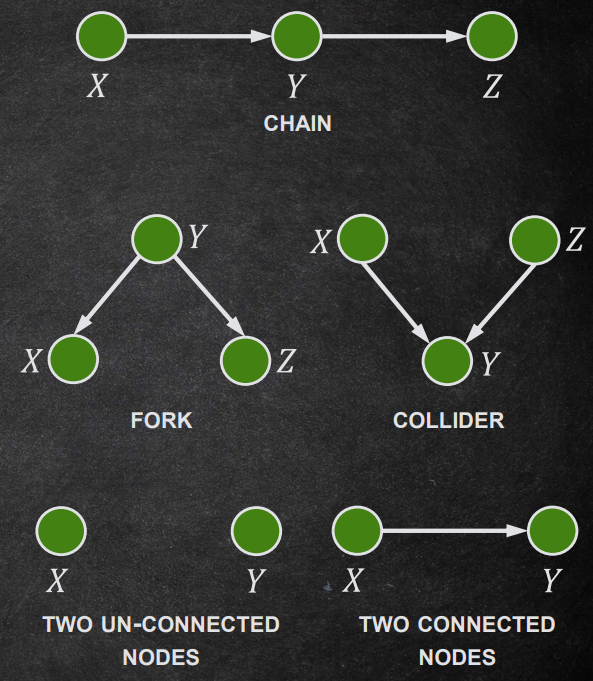
\includegraphics[width=0.7\textwidth]{img/basic_bn.png}
    \caption{Basic elements of a DAG}
\end{figure}

By flow of association, we mean whether any two nodes in a graph are associated
or not associated. In other terms, we want to know whether two nodes are
(statistically) dependent or (statistically) independent. However, we will also
study whether two nodes are conditionally independent or not.
\subsection{Two un-connected nodes}
Given a graph consisting of just two unconnected nodes, these nodes are not
associated, because there is no edge between them. To show this, consider the
factorization of the joint probability $P(X, Y)$ that the Bayesian network
factorization gives us: $P(X, Y) = P(X)P(Y)$. This factorization immediately
gives us a proof that the two nodes are unassociated (independent).
\subsection{Two connected nodes}
On the contrary, if there is an edge between the two nodes, then the two nodes
are associated. We exploit the causal edges assumption which means that $X$ is
a direct cause of $Y$. They are dependent and conditional dipendent.
\subsection{Chain and Fork}
We can consider this two building blocks together, because they share the same
set of dependencies. In both cases, the association flows from $X$ to $Z$ through
$Y$.

They also share the same set of independencies. When we condition on $Y$ in both
graphs, it blocks the flow of association from $X$ to $Y$. Therefore, when we
condition on $Y$ ( $Z$'s parent in both graphs), $Z$ becomes independent of (and
viceversa). This independence is an instance of a \textbf{blocked path}.
\begin{note}
    The flow of association in general is symmetric, but the flow of causation
    is not.
\end{note}
\subsection{Collider}
Association flows along any path that does not contain a \textbf{collider}. A
collider is a node with two or more parents that are independent $X \perp Z$.
We can think of $X$ and $Z$ simply as unrelated events that can happen, and which
both contribute to some common effect ($Y$). To show that $X \perp Z$ we apply
the Bayesian network factorization and then marginalize out $Y$.

The collider $Y$ blocks the path from node $X$ to node $Z$ and blocks the path
from node $Z$ to node $X$. This is another example of a blocked path, but this
time the path is not blocked by conditioning; the path is un-blocked by conditioning
on a collider.

Conditioning on descendants of a collider also induces association in between the
parents of the collider. The intuition is that if we learn something about a
collider's descendant, we usually also learn something about the collider itself
because there is a direct causal path from the collider to its descendants, and
we know that nodes in a chain are usually associated assuming minimality.
\section{D-separation}
\begin{definition}[\textbf{D-separation}]
    A path $p$ is blocked by a set of nodes $S$ if and only if:
    \begin{itemize}
        \item $p$ contains a chain of nodes or a fork such that the middle node
              is in $S$.
        \item $p$ contains a collider such that the collision node is not in $S$,
              and no descendant of the collision node is in $S$.
    \end{itemize}
    If $S$ blocks \textbf{every} path between two nodes $X$ and $Y$, then $X$ and
    $Y$ are \textbf{d-separated}, conditional on $S$, and thus are independent
    conditional on $S$.
\end{definition}
D-separation is an extremely important concept, because it implies conditional
independence. This is a very powerful tool for reasoning about causal models.
\begin{itemize}
    \item $X \perp_G Y | S$ implies that $X$ and $Y$ are d-separated in the DAG
          $G$ when conditioning on $S$.
    \item $X \perp_P Y | S$ implies that $X$ and $Y$ are independent in the
          distribution $P$ when conditioning on $S$.
\end{itemize}
\begin{definition}[\textbf{Global Markov Assumption}]
    Given that $P$ is Markov with respect to a DAG $G$, if $X$ and $Y$ are d-separated
    in $G$ conditional on $S$, then $X$ and $Y$ are independent conditional on $S$.
\end{definition}

Not only is association not causation, but causation is a sub-category of
association, thus association and causation both flow along directed paths.

We can tell if two nodes are not associated by whether or not they are d-separated.

If we want to measure the causal effect of $X$ on $Y$, we need to ensure that $X$
and $Y$ are d-separated in the augmented graph where we remove outgoing edges
from $X$. This is the only way to ensure that the association we measure is causation.

\begin{note}
    Association is symmetric while causation not.
\end{note}

To summerizing every assumptions:
\begin{itemize}
    \item local/global Markov Assumption: tells us which nodes are unassociated, tells 
    along which paths the association doesn't flow
    \item Minimality assumption: tells us which paths association does flow along
    \item Causal edges assumption: tells us causation flows along directed paths.
\end{itemize}
\begin{figure*}[!h]
    \centering
    \includegraphics*[width=\textwidth]{img/causal_networks_assumptions.png}
\end{figure*}



\end{document}